\chapter{LINGUISTIQUE FONCTIONNELLE ET PHONOLOGIE}
\label{chapter-8}
\markright{Linguistique fonctionnelle et phonologie}
\origpage{218}{204}
\begin{keybox}[Plan du chapitre]
\small\setstretch{1.03}
\setlist{topsep=.15em,itemsep=.15em,parsep=0pt}
\renewcommand{\thempfootnote}{校\arabic{editorialnote}}
\textbf{I.\quad LES FONCTION DU LANGAGE}\ednote{章首提纲保留原字。LES FONCTION 应为 LES FONCTIONS；systématique fonctionnelle 应为 systémique fonctionnelle，与本章正文第 212 页的标题一致。章名按第 204 页原题转写。}\par
\begin{enumerate}[label=\arabic*.]
\item Le schéma de la communication
\begin{enumerate}[label=\textcircled{\scriptsize\arabic*}]
\item Destinateur et destinataire
\item Le message
\item Le canal (le contact)
\item Le contexte (le référent)
\item Le code
\end{enumerate}
\item Les fonctions du langage
\begin{enumerate}[label=\textcircled{\scriptsize\arabic*}]
\item Le classement de Karl Bühler
\begin{enumerate}[label=\arabic*.]
\item La fonction expressive
\item La fonction appellative
\item La fonction représentationnelle
\item La fonction argumentative
\item Hiérarchie et valeur des fonctions
\end{enumerate}
\item Le classement de Jakobson
\begin{enumerate}[label=\arabic*.]
\item La fonction émotive
\item La fonction dénotative (référentielle)
\item La fonction phatique
\item La fonction conative
\item La fonction poétique
\item La fonction métalinguistique
\end{enumerate}
\item Le classement de Michael Halliday
\begin{enumerate}[label=\arabic*.]
\item La grammaire systématique fonctionnelle
\item Les trois métafonctions du langage
\item Les sept fonctions du langage chez l’enfant
\end{enumerate}
\end{enumerate}
\end{enumerate}
\textbf{II.\quad LA PHONOLOGIE}\par
\begin{enumerate}[label=\arabic*.]
\item La linguistique fonctionnelle en France
\begin{enumerate}[label=\textcircled{\scriptsize\arabic*}]
\item André Martinet : un des plus grands linguistes du 20e siècle
\item La double articulation du langage
\item Phonétique et phonologie
\end{enumerate}
\origpage{219}{205}
\item La phonologie et ses unités
\begin{enumerate}[label=\textcircled{\scriptsize\arabic*}]
\item Phonématique et phonèmes
\item Prosodie et prosodèmes
\end{enumerate}
\item Les outils de la phonologie
\begin{enumerate}[label=\textcircled{\scriptsize\arabic*}]
\item Le corpus
\item La commutation
\item Les paires minimales
\end{enumerate}
\item Statut phonologique des sons
\begin{enumerate}[label=\textcircled{\scriptsize\arabic*}]
\item Les phonèmes
\item Les allophones
\begin{enumerate}[label=\arabic*.]
\item La variante libre
\item La variante contextuelle
\item Les allophones des tonèmes\par
1) Le \textit{sandhi} tonal\par
2) Le cas du mandarin
\end{enumerate}
\item Les archiphonèmes
\begin{enumerate}[label=\arabic*.]
\item La neutralisation
\item Archiphonème et allophone
\end{enumerate}
\end{enumerate}
\end{enumerate}
\textbf{Exercices}\par
\textbf{Pour aller plus loin}\par
\textbf{Glossaire}
\end{keybox}

\origpage{220}{206}
\begin{keybox}[Introduction]
\renewcommand{\thempfootnote}{校\arabic{editorialnote}}
Le cercle linguistique de Prague (« l’école de Prague ») est un mouvement de réflexion et d’analyse linguistique très influent au début du 20e siècle. Fondateur et premier président du Cercle, le linguiste tchèque Vilém Mathesius (1882-1945) défendait le principe d’une étude systématique, synchronique et immanente de la langue.

Les \textit{Travaux du cercle linguistique de Prague}, huit volumes publiés entre 1929 et 1939, ont été déterminants dans le domaine de la phonologie.Dans cet ouvrage, le terme de « structure » est apparu pour la première fois.\ednote{原文 phonologie.Dans 缺少句间空格，应为 phonologie. Dans。“structure 一词首次出现”的范围没有限定，此说仍需历史词例或原刊证据；不能把本句作为该词在所有学科中首次使用的依据。} En considérant que « la langue est un système fonctionnel » et en préconisant « une méthode propre à permettre de découvrir les lois de structure des systèmes linguistiques », les membres du Cercle ont ouvert le programme des études structurales en linguistique.

Quant à la notion de fonction dans le fonctionnalisme pragois est polysémique,\ednote{此句句法衔接有误：可改为 La notion de fonction dans le fonctionnalisme pragois est polysémique，或 Quant à la notion de fonction dans le fonctionnalisme pragois, elle est polysémique。正文保留原句。} elle peut être envisagée d’abord du point de vue du but de la communication : pour le Cercle, la langue, comme les autres produits de l’activité humaine, possède un caractère de finalité, c’est-à-dire qu’elle est utilisée en vue d’une fin. Mais la fonction est aussi ce qui permet de distinguer les signes ou leurs composants dans le système de la langue. C’est à ces deux aspects de la notion de fonction qu’est consacré ce chapitre : nous y présenterons les fonctions du langage, puis la phonologie, c’est-à-dire l’étude des sons du point de vue de leur « fonction ».
\end{keybox}

\section{LES FONCTIONS DU LANGAGE}
Lorsque l’on évoque les fonctions du langage, un nom s’impose : celui de Roman Jakobson, Né à Moscou en 1896,\ednote{原文在逗号后大写 Né。可断为 celui de Roman Jakobson. Né à Moscou en 1896, cofondateur…；这里不静默改变底本标点。} cofondateur du Cercle de Prague, il a été un des professeurs de \textbf{Noam Chomsky}. Au MIT, il a participé à la redécouverte de Charles Sanders Peirce et a joué un rôle très actif dans les travaux de l’Association internationale de sémiotique fondée en 1969. Il est considéré comme un des linguistes les plus influents du 20e siècle.

\subsection{Le schéma de la communication}
En 1960, dans \textit{Linguistique et poétique} (traduction française par Nicolas Ruwet, Éditions de Minuit, Paris, 1963.), Jakobson a élaboré un modèle linguistique très célèbre qui porte son nom : le « schéma de Jakobson ». Pour lui, « le langage doit être étudié dans toutes ses fonctions ». Autrement dit, la linguistique doit s’attacher à comprendre à quoi sert le langage. Pour cela, une connaissance préalable des facteurs constitutifs de tout acte de communication verbale, est nécessaire. Le schéma de Jakobson permet justement d’identifier tous les intervenants et tous les facteurs qui entrent en jeu dans une situation de communication, comme représenté ci-dessous :

\origpage{221}{207}
\begin{center}
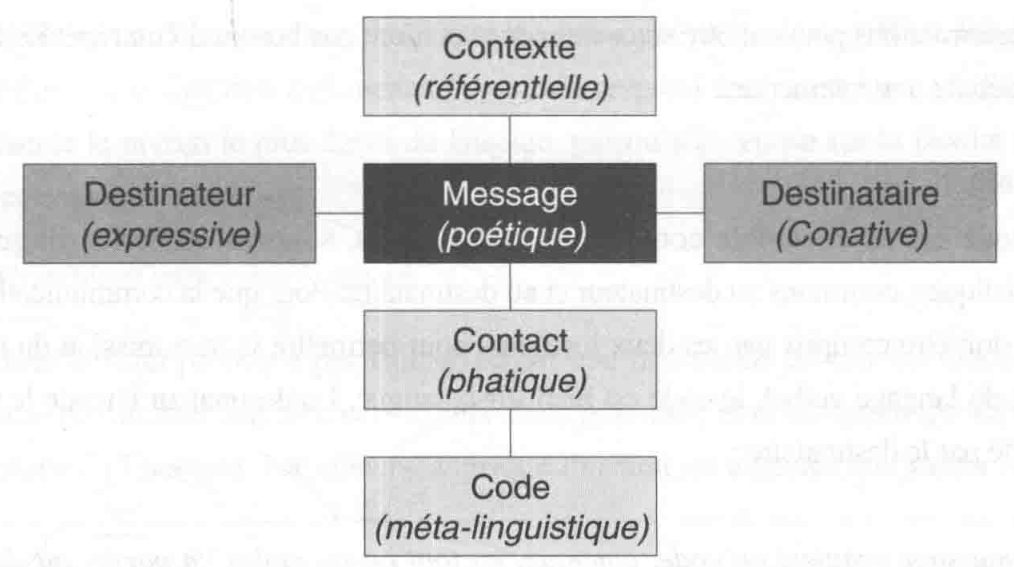
\includegraphics[width=.78\linewidth]{assets/ch08_communication_original.png}
\end{center}
\minititle{\textcircled{\scriptsize 1} Destinateur et destinataire}
Ils correspondent respectivement à l’émetteur et au récepteur, et le destinateur envoie un message au destinataire. Dans le cas d’une interaction normale, la communication est bidirectionnelle, et deux personnes interagissent de façon courante. Dans les cas où la communication est institutionnalisée, elle est unidirectionnelle et l’interaction implique l’intervention verbale d’une seule personne alors que l’autre écoute.\ednote{辨析：本句把制度化交际一概等同于单向交际，范围过宽。制度化访谈、审讯、课堂问答等在概念上都容许双方轮流发言；“制度化”与“是否双向”不是同一个分类维度。可改为“某些制度化传播情境主要是单向的”，而不能据本句排除制度化对话。}

\minititle{\textcircled{\scriptsize 2} Le message}
Il s’agit de l’information transmise par l’interlocuteur. Le message varie dans sa durée, sa forme et son contenu. Dans les interactions individualisées, le message est généralement adapté à l’interlocuteur. Dans les communications institutionnalisées (presse, télévision, publicité, etc.) le message est plutôt rigide et standard.

\minititle{\textcircled{\scriptsize 3} Le canal (le contact)}
Pour Jakobson, « le message requiert un contact, un canal physique et une connexion psychologique entre le destinateur et le destinataire, contact qui leur permet d’établir et de maintenir la communication ». Ce canal peut être direct, comme lors d’une discussion face à face. Il implique alors une réponse directe dans le même médium. Mais comme on dit : « Les paroles s’envolent, les écrits restent. » Le canal peut être modifié pour vaincre l’effet du temps. Dans ce cas là, le canal est indirect et la communication médiatisée passe des supports papier (livre, journal , magazine, etc.), ou numériques (WeChat, email, etc.).\ednote{原文 passe des supports 缺少介词，应为 passe par des supports。ce cas là 的规范连写为 ce cas-là。此处仅指出文字问题，不改动原段。}

\minititle{\textcircled{\scriptsize 4} Le contexte (le référent)}
Le contexte de situation réfère aux informations communes aux deux locuteurs sur la situation au moment de la communication :
\begin{quote}\small\itshape
Pour être opérant, le message requiert d’abord un contexte auquel il renvoie (c’est ce qu’on appelle aussi, dans une terminologie quelque peu ambiguë, le référent), contexte saisissable par le destinataire, et qui est soit verbal, soit susceptible d’être verbalisé.
\end{quote}
\origpage{222}{208}
Ces informations peuvent être sous-entendues et n’ont pas besoin d’être répétées à chaque fois que l’on débute une interaction.

\minititle{\textcircled{\scriptsize 5} Le code}
Un code est un ensemble conventionnel de signes, sonores ou écrits, linguistiques ou non linguistiques, communs au destinateur et au destinataire. Pour que la communication s’établisse, ce code doit être compris par les deux locuteurs pour permettre la transmission du message. Dans le cadre du langage verbal, le code est bien sûr la langue. Le destinateur encode le message qui sera décodé par le destinataire :
\begin{quote}\small\itshape
Le message requiert un code, commun, en tout ou au moins en partie, au destinateur et au destinataire (ou, en d’autres termes, à l’encodeur et au décodeur du message).
\end{quote}

\subsection{Les fonctions du langage}
Le nombre de fonctions du langage reconnues a varié selon les théories linguistiques. Commençons par présenter les travaux de Karl Bühler, un proche du Cercle de Prague.

\minititle{\textcircled{\scriptsize 1} Le classement de Karl Bühler}
\textbf{Karl Bühler} (1879-1963) est un psychologue, professeur et théoricien du langage allemand. Constatant que tout énoncé dans un acte de discours entretient une triple relation avec l’état de choses dont on parle, le sujet parlant et celui à qui l’on parle, Karl Bühler a dégagé trois fonctions fondamentales du langage : la fonction d’expression , de représentation, et d’appel, renommées plus tard fonction expressive, représentationnelle et appellative.

\minititle{1. La fonction expressive}
La fonction expressive consiste à signifier les états intérieurs psychiques ou moraux des animaux et des êtres humains, ce qui correspond à la \textit{phônè} d’Aristote.

\minititle{2. La fonction appellative}
La fonction appellative est parfois appelée fonction de signal. En communiquant un message, l’émetteur, homme ou animal, tente de provoquer une réaction chez le récepteur.

\minititle{3. La fonction représentationnelle}
Cette fonction forme la majeure partie de la communication humaine. Lorsque nous communiquons, nous décrivons nos expériences à autrui. Cette fonction de description se distingue par la possibilité qu’ont les énoncés factuels d’être vrais ou faux. Le mensonge, en tant que spécificité humaine, est une possibilité implicite.

\minititle{4. La fonction argumentative}
La fonction argumentative ne figurait pas dans la triade originelle de Bühler. Elle a été ajoutée \origcont{223}{209}en 1953 par un de ses anciens étudiants, le philosophe des sciences \textbf{Karl Popper} (1902-1994). Pour Popper, la fonction argumentative, qui correspond à la discussion critique, à la rhétorique représente le niveau le plus élevé du langage, puisqu’elle repose sur la faculté qu’a l’homme de penser rationnellement.

\minititle{5. Hiérarchie et valeur des fonctions}
La classification proposée par Bühler établit une hiérarchie entre deux fonctions primaires de langage communes aux animaux et aux êtres humains, et deux fonctions supérieures qui sont l’apanage de l’homme.\ednote{本段“四种功能”的归属与上段矛盾：上段已说明 Bühler 原为三分法，第四项由 Popper 增补。因而此处应限定为“经 Popper 扩充的分类”，不能把四项均归于 Bühler 原始三分法。有关 1953 年和下列价值配对的具体原刊页码，仍待核。} Par ailleurs, à chaque fonction est associée une valeur en lien avec le but visé :
\begin{itemize}
\item Fonction argumentative : un argument sera soit pertinent, soit non pertinent.
\item Fonction de description : une description sera soit vraie, soit fausse.
\item Fonction de signal : un signal sera soit efficace, soit inefficace.
\item Fonction expressive : le destinateur sera soit éloquent, soit non éloquent.
\end{itemize}

\minititle{\textcircled{\scriptsize 2} Le classement de Jakobson}
S’appuyant sur cette première classification, Jakobson a ajouté d’autres éléments. En tenant compte des six éléments présentés plus haut dans son schéma de la communication, il distingue six fonctions du langage : « Chacun de ces six facteurs donne naissance à une fonction linguistique différente. »

\minititle{1. La fonction émotive}
La fonction émotive est utilisée par le destinateur pour informer le récepteur sur sa propre personnalité ou ses propres pensées. Dans l’ouvrage cité plus haut à plusieurs reprises, Jakobson la définit ainsi :
\begin{quote}\small\itshape
Elle vise à une expression directe de l’attitude du sujet à l’égard de ce dont il parle. Elle tend à donner l’impression d’une certaine émotion, vraie ou feinte ; c’est pourquoi la dénomination de fonction émotive [...] s’est révélée préférable à fonction émotionnelle. La couche purement émotive, dans la langue, est représentée par les interjections.
\end{quote}

\begin{bbcomplement}{}
Pour illustrer la fonction expressive, Jakobson raconte l’anecdote d’un acteur qui s’était rendu chez le metteur en scène Constantin Stanislavski (1863-1938) pour passer une audition en vue d’obtenir un rôle. Lors de cette audition, Stanislavski lui a demandé de répéter quarante fois l’expression \textit{segodnya večerom} (« ce soir », en russe), en variant à chaque fois l’intonation. Pour que l’audition soit réussie, il fallait que \origcont{224}{210}l’auditoire puisse reconnaître chacune de ces situations « à partir des changements dans la configuration phonique de ces deux simples mots ».

Un ancien acteur du théâtre de Stanislavski à Moscou m’a raconté comment, quand il passa son audition, le fameux metteur en scène lui demanda de tirer quarante messages différents de l’expression Segodnja vecerom, « Ce soir », en variant les nuances expressives. Il fit une liste de quelque quarante situations émotionnelles et émit ensuite l’expression en question en conformité avec chacune de ces situations, que son auditoire eut a reconnaître uniquement a partir des changements dans la configuration phonique de ces deux simples mots.\ednote{引文此处两个 a 均应为介词 à：eut à reconnaître、à partir。另，正文两处俄语拉丁转写形式不同，均依底本保留，不以统一转写静默替换。} Dans le cadre des recherches que nous avons entreprises [...] sur la description et l’analyse du russe courant contemporain, nous avons demandé à cet acteur de répéter l’épreuve de Stanislavski. Il nota par écrit environ cinquante situations impliquant toutes cette même phrase elliptique et enregistra sur disque les cinquante messages correspondants. La plupart des messages furent décodés correctement et dans le détail par des auditeurs d’origine moscovite.
\end{bbcomplement}

\minititle{2. La fonction dénotative (référentielle)}
Le concept de dénotation ne nous est pas inconnu. La fonction dénotative, centrée sur le référent, établit une relation entre le message et l’objet auquel il renvoie. Utilisée pour donner une information, décrire la réalité, rapporter objectivement un événement, elle consiste à parler « de ». Cette fonction est prédominante dans le récit, la poésie épique, les documents publicitaires, les textes de loi, etc.

\minititle{3. La fonction phatique}
L’adjectif « phatique » vient du grec ancien \textit{phatis}, qui signifie « parole ». Il a d’abord été utilisé par l’anthropologue polonais \textbf{Bronisław Malinowski} (1884–1942) dans avant d’être repris\ednote{原文 dans avant d’être repris 中 dans 后无成分，句子残缺。若仅作语法修复可删去 dans；若原本拟列著作名称或日期，则须另据底本补证。本版不臆补缺文。} en linguistique par Roman Jakobson, qui le définit ainsi :
\begin{quote}\small\itshape
Il y a des messages qui servent essentiellement à établir, prolonger ou interrompre la communication, à vérifier si le circuit fonctionne (« Allô, vous m’entendez ? »), attirer l’attention de l’interlocuteur ou à s’assurer qu’elle ne se relâche pas (« Dites, vous m’écoutez ? » ou, en style shakespearien, « Prêtez-moi l’oreille ! ») - et, à l’autre bout du fil, « Hm-hm ! »).
\end{quote}
On voit que la fonction phatique porte sur le canal. Jakobson précise que la fonction phatique désigne aussi « la tendance à communiquer (qui) précède la capacité d’émettre ou de recevoir des messages porteurs d’information ». Certains linguistes font entrer dans cette catégorie les discussions mondaines, tous les artifices de langages (anecdotes, histoires drôles, parler de la pluie et du beau temps) utilisés pour maintenir le contact verbal sans défaillance et éviter que s’installent une gêne, un silence.

\minititle{4. La fonction conative}
Nous avons, dès le premier chapitre, évoqué la conation, définie comme une impulsion dirigée \origcont{225}{211}vers un passage à l’action. La fonction conative exerce une visée intentionnelle sur le destinataire et cherche à avoir sur lui un certain effet. Parler c’est agir sur les autres. Les ordres, les défenses, les plaidoiries, les prédications, les conseils, les exhortations, les requêtes, les promesses n’en sont quelques illustrations.\ednote{原文 n’en sont quelques illustrations 缺少 que，应为 n’en sont que quelques illustrations。} C’est une fonction privilégiée en publicité et en politique : toute la rhétorique est basée sur la fonction conative du langage.

\minititle{5. La fonction poétique}
On sait que c’est par la poésie que Jakobson est arrivé à la phonologie. Toujours dans l’ouvrage cité plus haut, il définit ainsi la fonction poétique :
\begin{quote}\small\itshape
La visée du message en tant que tel, l’accent mis sur le message pour son propre compte, est ce qui caractérise la fonction poétique du langage. Cette fonction ne peut être étudiée avec profit si on perd de vue les problèmes généraux du langage [...]. La fonction poétique n’est pas la seule fonction de l’art du langage, elle en est seulement la fonction dominante, déterminante, cependant que dans les autres activités verbales elle ne joue qu’un rôle subsidiaire, accessoire.
\end{quote}

\begin{bbcomplement}{}
Pour illustrer la fonction poétique, on songera à Jean-Paul Sartre (1905-1980) qui, dans \textit{Qu’est-ce que la littérature ?} (1947), a écrit : « la prose se sert de mots, la poésie sert les mots ». Jakobson précise que la notion de fonction poétique n’est pas spécifique au domaine poétique et qu’elle concerne les communications quotidiennes :
L’étude linguistique de la fonction poétique doit outrepasser les limites de la poésie, et, d’autre part, l’analyse linguistique de la poésie ne peut se limiter à la fonction poétique.
\end{bbcomplement}

\minititle{6. La fonction métalinguistique}
La fonction métalinguistique fait appel à la capacité qu’a la langue de pouvoir expliciter ses propres codes, ses propres règles et son propre lexique : elle est centrée sur le code.

Cette fonction est un peu particulière, car parmi tous les systèmes de signes, le langage est le seul à pouvoir se prendre comme propre référent. À l’écrit, les définitions, les explications, les commentaires, les corrections, les traductions, etc. reposent sur cette fonction. etc.\ednote{句末 fonction. etc. 的 etc. 与前面的 etc. 重复，且单独成残句；应删去后一个 etc.。} À l’oral, elle se manifeste à travers l’utilisation d’expressions comme « ce que je veux dire », « en d’autres termes », etc.

\begin{bbcomplement}{}
L’épanorthose, figure de style qui consiste à corriger une affirmation jugée trop faible en y ajoutant une expression plus frappante, est une illustration de la fonction métalinguistique, comme dans la célèbre « tirade du nez » de \textit{Cyrano de Bergerac} d’Edmond Rostand (1868-1918) :

« C’est un roc ! ... C’est un pic ... C’est un cap ! Que dis-je, c’est un cap ? ... C’est une péninsule ! »
\end{bbcomplement}

\origpage{226}{212}
Une dernière remarque avant de quitter Jakobson : il considère que les six fonctions présentées au-dessus ne s’excluent pas les unes les autres, mais que souvent elles se superposent. Le langage peut ainsi servir à plusieurs choses à la fois : par, maintenir par exemple le contact (fonction phatique) tout en prenant pour objet le code du message (fonction métalinguistique).\ednote{原文 par, maintenir 中 par, 为赘文，拟删为 … à la fois : maintenir par exemple…；不据此改动正文。} « Vous voyez ce que je veux dire ? »

\minititle{\textcircled{\scriptsize 3} Le classement de Michael Halliday}
Née de la rencontre entre le fonctionnalisme et la grammaire, la théorie de la grammaire fonctionnelle a été initialement développée par \textbf{Simon Dik} (1940-1995), linguiste néerlandais, dans un ouvrage posthume : \textit{The Theory of Functional Grammar} a publié en 1997.\ednote{a publié 应为 publié（过去分词修饰 ouvrage），或改写为 qui a été publié。出版社将 1997 年第一卷明确标为第二次修订版，不能把该身后版本的年份直接等同于理论首次发展的年份。Dik 与 Halliday 的具体理论影响关系，仍待核。\ecite{48}} De son point de vue, la grammaire est un instrument d’interaction sociale entre êtres humains. Mettant l’accent sur la fonction de communication, Dik définit ainsi la grammaire fonctionnelle :
\begin{quote}\small\itshape
D’un point de vue fonctionnel, une langue est tout d’abord un modèle de référence conceptualisé comme un instrument d’interaction social entre êtres humains, avec pour objectif d’établir des relations communicantes. C’est alors que l’on peut tenter de révéler l’instrumentalité linguistique dans les limites du possible en veillant à respecter l’utilisation et l’objectif de ces termes lors d’interactions sociales. En d’autres termes, le langage naturel fait partie intégrante de la compétence de communication.
\ednote{引文 instrument d’interaction social 中形容词若修饰 interaction，应为 sociale。该法语译文的原始出处待核。}
\end{quote}

\minititle{1. La grammaire systémique fonctionnelle}
La théorie de Dik a reçu d’importants apports de la grammaire systémique fonctionnelle de \textbf{Michael Halliday} (1925-2018) un des linguistes contemporains les plus influents en Grande-Bretagne. Le modèle de Halliday est appelé systémique car il s’apparente, sur le plan des règles et des mécanismes, au fonctionnement d’un ordinateur.\ednote{待核：底本将 systémique 这一名称的缘由直接归于计算机运作类比，却未列该句出处。这一归因仍需 Halliday 原著支持，不能仅据类比确证术语史。} Le postulat de base est le suivant :
\begin{quote}\small\itshape
The explanation of how language works needs to be grounded in a functional analysis, since language has evolved in the process of carrying out certain critical functions as human beings interacted with their eco-social environment.
\end{quote}

\minititle{2. Les trois métafonctions du langage}
Michael Halliday distingue trois fonctions principales du langage, qu’il appelle \textit{metafunctions} (métafonctions) :
\begin{itemize}
\item la fonction idéationnelle (\textit{ideational function}), qui a pour objet la représentation de l’expérience, qui permet de décrire les phénomènes du monde réel, extérieur à nous ou intérieur.
\item la fonction interpersonnelle (\textit{interpersonal function}), qui s’exerce dans la relation sociale de communication, qui permet au locuteur de participer à un échange verbal.
\item la fonction textuelle (\textit{textual function}), qui consiste à créer du texte : « create coherent text \origcont{227}{213}– text that coheres within itself and with the context of situation.» Fonction proprement linguistique, elle permet aux deux autres fonctions de prendre forme à travers toutes les ressources du système grammatical.
\end{itemize}

\minititle{3. Les sept fonctions du langage chez l’enfant}
Selon Halliday, les fonctions du langage sont distinctes chez les enfants selon qu’ils utilisent le langage pour faire (\textit{language as doing}) ou pour apprendre (\textit{language as learning}). En 1975, dans \textit{Learning how to mean}, il a identifié sept fonctions dans le langage des enfants :
\begin{itemize}
\item La fonction instrumentale, qui sert à manipuler l’environnement, à faire en sorte que certains événement se produisent.\ednote{certains événement 应为 certains événements，名词须用复数。}\par
\textbf{Ex :} \textit{Want juice}
\item La fonction de régulation, qui tend à contrôler les événements, dire aux autres quoi faire.\par
\textbf{Ex :} \textit{Go away!}
\item La fonction d’interaction, qui sert à créer des contacts, à établir des liens avec son entourage.\par
\textbf{Ex :} \textit{Love you, Mummy.}
\item La fonction personnelle, qui sert à exprimer ses émotions, ses opinions et sa personnalité.\par
\textbf{Ex :} \textit{Me good girl}
\end{itemize}
Les trois fonctions suivantes aident l’enfant à comprendre son environnement. C’est ce que Halliday appelle \textit{language as learning} :
\begin{itemize}
\item La fonction de représentation, qui utilise le langage pour transmettre des faits, des connaissances, expliquer, rapporter la réalité :\par
\textbf{Ex :} \textit{Daddy’s angry.}
\item La fonction heuristique, utilisée pour acquérir des connaissances sur son environnement :\par
\textbf{Ex :} \textit{What is the tractor doing?}
\item La fonction imaginative, utilisée pour créer des systèmes ou des idées de l’imagination, raconter des histoires.
\end{itemize}

\section{LA PHONOLOGIE}
Le point de départ des travaux du Cercle de Prague réside dans la distinction, établie par Troubetzkoy et Jakobson, entre phonétique et phonologie. La deuxième thèse du \textit{Manifeste du Cercle de Prague} (1928) dont ils étaient tous deux coauteurs jugeait nécessaire de « distinguer le son comme fait physique objectif, comme représentation et comme élément du système fonctionnel ». Selon eux, on doit faire la différence, dans le \origcont{228}{214}matériau de la langue, entre les sons qui autorisent des différenciations sémantiques (les phonèmes) et ceux dont les variations ne sont associées à aucune différenciation sémantique. L’effort tend ici vers une définition fonctionnelle strictement linguistique : Les \textit{Principes de phonologie historique} (1931) de Jakobson, ainsi que \textit{La Phonologie actuelle} (1933) et les \textit{Principes de phonologie} (1939) de Troubetzkoy ont fondé la phonologie.

\subsection{La linguistique fonctionnelle en France}
Lorsque l’on évoque la phonologie et le fonctionnalisme en France, impossible de ne pas évoquer le linguiste \textbf{André Martinet} (1908-1999).

\minititle{\textcircled{\scriptsize 1} André Martinet : un des plus grands linguistes du 20e siècle}
André Martinet est le père de l’analyse fonctionnaliste en linguistique française. Séduit par les conceptions de l’école de Prague, Martinet a rencontré Troubetzkoy de passage à Paris en 1933 et a commencé à entretenir une correspondance avec lui. En 1934, il a épousé une Danoise, et ses séjours à Copenhague l’ont conduit à nouer des relations avec le sémiologue \textbf{Louis Hjelmslev} (1899-1965), pionnier du structuralisme et continuateur de Saussure. Agrégé d’anglais, André Martinet a enseigné à l’Université de Columbia aux États-Unis, où il a été nommé directeur du département de linguistique (1947-1955) avant de devenir directeur de la célèbre revue \textit{Word}. Président de la Société européenne de linguistique (1966-1999),\ednote{任期误。SLE 官方历史页所录首任会长为 1966 年的 André Martinet，任至 1967 年年会；1967 年已由 Björn Collinder 接任。原文不能把 1966–1999 当作连续会长任期。\ecite{45}} fondateur de la Société de linguistique fonctionnelle et de la revue \textit{La Linguistique}, son ouvrage \textit{Langue et Fonction} (1962) a marqué les débuts de la syntaxe fonctionnelle. Son ouvrage le plus connu, \textit{Éléments de linguistique générale} (1960) a été traduit dans dix-sept langues et a influencé toute une génération de linguistes en France et dans le monde.

\minititle{\textcircled{\scriptsize 2} La double articulation du langage}
Inscrite dans le cadre de la linguistique fonctionnelle d’André Martinet, la double articulation désigne la propriété de tout énoncé linguistique d’être segmenté à deux niveaux : à un premier niveau (la première articulation), les unités ont à la fois une face formelle (le signifiant) et une face significative (le signifié). À un second niveau (la seconde articulation), les unités peuvent elles-mêmes être segmentées en unités plus petites n’ayant pas de sens, mais participant à la distinction du sens des unités de première articulation : ces unités distinctives sont appelées phonèmes. Cette double articulation constitue le fondement d’une économie importante dans la production d’énoncés linguistiques : en effet, avec un nombre limité de phonèmes (une trentaine en moyenne dans chaque langue), on peut construire un nombre illimité d’unités de première articulation et donc un nombre illimité d’énoncés.

\minititle{\textcircled{\scriptsize 3} Phonétique et phonologie}
L’étymologie de la phonologie se confond avec celle de la phonétique. Mais si phonologie et phonétique se consacrent toutes deux à l’étude des sons, elles ne l’abordent pas du même point de vue :
\begin{itemize}
\item La phonétique s’intéresse aux sons en tant qu’unités physiques et physiologiques concrètes, \origcont{229}{215}appelées « phones », elle n’intègre pas leur rôle au niveau de la sémantique.
\item La phonologie, à l’opposé, envisage les sons comme des entités abstraites, linguistiques, et du point de vue de leur rôle fonctionnel dans la langue : la dimension sémantique est dès lors fondamentale. C’est pour cela que la phonologie est parfois appelée « phonétique fonctionnelle ».
\end{itemize}
En fait, phonétique et phonologie sont complémentaires : la première étudie la matérialité des sons, la seconde étudie leur fonction. Troubetzkoy résume cela ainsi : la phonétique est « la science des sons de la parole » ; la phonologie est « la science des sons de la langue ».

\subsection{La phonologie et ses unités}
La phonologie, en recherchant des unités distinctives non significatives introduisant une différence de sens, a identifié deux types d’unités fonctionnelles : les phonèmes et le prosodèmes.\ednote{le prosodèmes 应为 les prosodèmes，冠词与复数名词须一致。} Chacun fait l’objet d’un domaine spécifique de la phonologie.

\minititle{\textcircled{\scriptsize 1} Phonématique et phonèmes}
La phonématique est le domaine de la phonologie qui vise à déterminer, parmi les sons inventoriés par la phonétique, ceux qui sont dotés d’une fonction distinctive. La phonématique traite les sons comme des unités se succédant sur l’axe horizontal de la chaîne parlée. Dans \bipa{[bato]}, \bipa{[rato]} et \bipa{[gato]}, les phonèmes \bipa{/b/}, \bipa{/r/} et \bipa{/g/} sont des unités distinctives qui servent à distinguer le sens des trois unités lexicales « bateau », « rateau » et « gâteau ».\ednote{法语词 rateau 缺少长音符，应为 râteau。音标中的元音选取依底本保留，不把某一地区的元音合流分析强加给所有法语变体。} Pour leur notation, on adopte des barres obliques (\bipa{/ /}), ce qui les différencie des phones de la phonétique représentés entre crochets (\bipa{[ ]}).

\minititle{\textcircled{\scriptsize 2} Prosodie et prosodèmes}
Dans certaines langues, d’autres unités que les phonèmes peuvent être dotées d’une fonction distinctive. La prosodie est le domaine de la phonologie qui porte sur ces unités, appelées « prosodèmes » ou « traits suprasegmentaux », c’est-à-dire des traits phonétiques qui se superposent à la chaîne linéaire constituée par les phonèmes (les traits segmentaux). Parmi les unités que la prosodie étudie, on compte (entre autres) les prosodèmes suivants : l’accent, le rythme, l’intonation, le timbre, l’accent tonique, ou encore le ton (appelé « tonème » en phonétique) dans le cas des langues tonales.\ednote{术语层级有误：按本段和随后定义，具有区别功能的声调单位 tonème 属于音系分析，应将 en phonétique 改为 en phonologie。音色 timbre 也不能不加限定地全算为超音段特征；如元音音质同时用于区分音段。参见官方 IPA 表对元音、超音段特征和声调的分别列示。\ecite{41}}

Les tonèmes sont des unités prosodiques distinctives consistant principalement en une modification de la hauteur de la voix. À la différence des phonèmes, les tons ne sont pas segmentables : l’unité tonale ne peut en effet être perçue sans le support des phonèmes et n’existe donc pas sans eux. Ce sont donc littéralement des unités suprasegmentales. On pourrait dire que les tonèmes sont des phonèmes propres aux langues tonales.

\origpage{230}{216}
\begin{bbcomplement}{Langue tonale}
Fait peu connu, soixante à soixante-dix pour cent des langues du monde sont tonales et presque toutes sont non-européennes.\ednote{统计与范围提示：这里未注明估计的抽样框及“声调语言”口径，不宜作为精确普查比例。WALS 第 13 章明确提醒其样本不按各地区语言密度比例取样，并将挪威语等欧洲语言列入声调或边缘声调类。因此，既不能由该样本直接推出全球比例，也不能把声调限定为非欧洲现象。底本估计保留，不用另一口径的新数字替换。\ecite{44}} On peut citer les langues d’Asie du Sud-Est, d’Extrême-Orient, les langues chinoises (mandarin, cantonais, min, gan, hakka...), les langues tai (thaï, lao, shan, zhuang), le birman, etc. Le thaï possède cinq tonèmes, le vietnamien en possède six. Le record, si je puis dire, appartient à la langue \textit{kam}, langue de l’ethnie Dong (侗族) parlée dans quelques endroits de la province du Guizhou et du Guangxi en Chine, et qui compte quinze tons.\ednote{待核：“十五调”以及“最高纪录”未指明侗语方言、调类与实际调值的计数口径，不能当作该语言所有变体共同的音位数。越南语“六调”的适用方言也须限定；具体数值须据各方言的原始描写核对。} Presque toutes les langues en Afrique au sud du Sahara sont également tonales. Le swahili est un rare exemple de langue africaine non tonale.
\end{bbcomplement}

\subsection{Les outils de la phonologie}
Revenons en Europe. Les linguistes du Cercle linguistique de Prague, réunis autour de Nicolas Troubetzkoy et de Roman Jakobson, ont donné dans les années 1930 à la phonologie une méthode et des outils tellement efficaces et rigoureux qu’ils sont devenus la référence dans les études structuralistes.

\minititle{\textcircled{\scriptsize 1} Le corpus}
Le corpus désigne le matériau sur lequel travaille le phonologue. C’est un échantillon de données linguistiques répondant à un critère de représentativité linguistique. Destiné à l’analyse linguistique, il doit permettre la généralisation et la formulation de lois. Cet « échantillon phonique », après avoir été sélectionné puis organisé, fait l’objet d’une transcription phonétique avant d’être soumis à l’analyse phonologique dont l’outil principal est la commutation.

\minititle{\textcircled{\scriptsize 2} La commutation}
La commutation désigne le procédé par lequel la phonologie identifie les phonèmes. D’un point de vue pratique, cette opération consiste à substituer (commuter) un son à un autre, pour savoir si ce son permet de distinguer des unités significatives, comme par exemple les sons \bipa{/p/} et \bipa{/b/} dans les unités lexicales « pain » et « bain ». La méthode de commutation est l’un des outils fondamentaux du fonctionnalisme d’André Martinet.

\minititle{\textcircled{\scriptsize 3} Les paires minimales}
En phonologie, une paire minimale est une paire d’unités lexicales dont le signifiant ne diffère que par un phonème et dont le signifié est différent. Par exemple, en français, « sapin » et « lapin », ne se distinguent que par leur initiale. Le phonologue posera l’existence de deux phonèmes distincts, \bipa{/s/} et \bipa{/l/}, puisque la substitution de phonème (commutation) entraîne une distinction de sens. Autre exemple : « père » (\bipa{[pɛʁ]}) et « mère » (\bipa{[mɛʁ]}) forment aussi une paire minimale qui permet d’identifier \bipa{/p/} et \bipa{/m/} comme des phonèmes distincts. Dans une approche structurale, c’est par la méthode de la paire minimale que s’opère l’identification des phonèmes.

\origpage{231}{217}
L’extrait ci-dessous, tiré de \textit{Zur allgemeinen Theorie der phonologischen Vokalsysteme} (« la théorie générale des systèmes vocaux phonologiques ») de \textbf{Nicolaï Troubetzkoy}, publié en 1929, nous rappelle de façon utile la différence entre phonétique et phonologie et illustre la notion de paire minimale avec deux exemples tirés de l’allemand :
\begin{quote}\small\itshape
Contrairement à la phonétique, qui est une science de la nature et traite des sons du discours humain, la phonologie a pour objet les phonèmes, soit les représentations mentales des sons du langage humain, et elle est à ce titre une branche de la linguistique.[...] Par ces associations phoniques avec divers autres mots de la même langue, le mot en question, ou plus exactement, la représentation de mot en question, est décomposée en ses constituants phonologiques, à savoir les représentations phoniques isolées ou phonèmes. Mais l’analyse associative n’en reste pas aux phonèmes isolés. Si on compare par exemple le mot allemand Keil, « coin », « cale », au mot Geil, « lubrique », on remarque qu’il y a entre les deux exactement la même différence qu’entre Pein, « douleur », et Bein, « jambe ».
\end{quote}

\subsection{Statut phonologique des sons}
Le but premier dans une analyse phonologique, on le sait à présent, est de déterminer si des différences phonétiques engendrent des différences sémantiques. En fonction de leurs propriétés, les sons peuvent avoir trois statuts phonologiques différents.

\minititle{\textcircled{\scriptsize 1} Les phonèmes}
Le phonème est une unité distinctive dépourvue elle-même de sens, mais qui induit une différence de sens dans le mot qui le contient : on l’a vu peu plus haut avec \bipa{[bato]}, \bipa{[rato]} et \bipa{[gato]}. L’espagnol compte 34 phonèmes, le français 36, l’italien 42, l’anglais 44, l’allemand 68.\ednote{这些音位数没有注明语言变体及分析口径，不能视为各语言唯一而固定的值。是否将长短对立、双元音、塞擦音等计作独立单位也会改变结果。这组数值的原始清单与口径仍待核。}

\minititle{\textcircled{\scriptsize 2} Les allophones}
Avec des allophones, la substitution d’un son à un autre ne modifie pas le sens du mot : les locuteurs leur attribuent le même rôle fonctionnel en phonologie, même s’ils perçoivent la différence phonétique entre les deux. Par exemple en français, le mot « père » peut diversement se prononcer : \bipa{[pɛr]}, \bipa{[pɛʀ]} ou \bipa{[pɛʁ]}. Autrement dit, il y a trois prononciations possibles du phonème \bipa{/r/}. En utilisant la terminologie du chapitre précédent, on distingue :
\begin{itemize}
\item \bipa{[r]} : consonne roulée alvéolaire
\item \bipa{[ʀ]} : consonne roulée apicale\ednote{发音部位误：\bipa{[ʀ]} 是小舌颤音（roulée uvulaire），不是舌尖颤音（apicale）；\bipa{[r]} 则是齿龈颤音。符号依底本保留，名称在此订正。\ecite{41}}
\item \bipa{[ʁ]} : consonne fricative uvulaire
\end{itemize}
Ces trois phones sont phonétiquement des sons différents mais leur différence n’est pas \textit{fonctionnellement} pertinente, puisque le sens perçu est le même. Ce sont des variantes de prononciation d’une même unité phonologique, le phonème \bipa{/r/}. Cette variante est appelée allophone, réalisation sonore possible (mais non distinctive) d’un même son.\ednote{按此处定义，allophone 是“同一音位”的不同语音实现，应将 d’un même son 改为 d’un même phonème，避免把具体语音与音位混为一谈。依据为本章前述音段／音位区分。} Les allophones sont \origcont{232}{218}des unités phonétiques et non phonologiques : ils sont donc écrits entre crochets. Mais attention : en arabe, les sons \bipa{[r]} et \bipa{[ʀ]} s’opposent et constituent donc deux phonèmes distincts.\ednote{待核：此处“阿拉伯语”未指明变体，也没有给出验证 \bipa{[r]／[ʀ]} 对立的最小对立语料。\bipa{[ʀ]} 和小舌擦音 \bipa{[ʁ]} 不能仅因形近而互换。原书可能混淆了颤音与擦音符号，本版不未经方言和语料核实就代换该例。\ecite{41}} Il existe deux types d’allophone : la variante libre et la variante combinatoire (appelée aussi contextuelle).

\minititle{1. La variante libre}
On parle de variante libre lorsque l’usager a la possibilité d’utiliser plusieurs allophones sans changer le sens de l’énoncé. Dans ce cas là, les différentes formes d’un phonème peuvent dépendre de l’origine géographique ou sociale du locuteur. Par exemple, si vous écoutez les \textit{Roses de Picardie}, célèbre chanson interprétée par le chanteur corse \textbf{Tino Rossi}, vous l’entendrez « rouler les r », autrement dit, prononcer le phonème \bipa{/r/} avec une consonne roulée alvéolaire. En revanche, si c’est moi qui chante, vous entendrez un \bipa{[ʁ]} standard, c’est-à-dire une consonne fricative uvulaire.

\minititle{2. La variante contextuelle}
Dans le cas de la variante contextuelle, et comme son nom l’indique, les formes différentes que peut prendre un même phonème dépendent nécessairement du contexte. Les formes ainsi identifiées s’excluent mutuellement dans un environnement (contexte linguistique) donné. En allemand, par exemple, le phonème \bipa{/x/} (dont la graphie est « ch ») est réalisé deux manières :\ednote{est réalisé deux manières 缺少介词，应为 est réalisé de deux manières。}
\begin{itemize}
\item avec le son \bipa{[x]}, consonne fricative vélaire sourde, après une voyelle ou diphtongue postérieure, comme dans \textbf{\textit{kochen}} (« cuire »), \textbf{\textit{Rauch}} (« fumée »), \textbf{\textit{acht}} (« huit »).
\item avec le son \bipa{[ç]}, consonne fricative palatale sourde, dans les autres positions : \textbf{\textit{Ich}} (« je »), \textbf{\textit{Licht}} (lumière), \textbf{\textit{Dolch}} (poignard), \textbf{\textit{Chemie}} (chimie), etc.
\end{itemize}

\minititle{3. Les allophones des tonèmes}
Si les allophones concernent principalement les traits segmentaux, ils peuvent également concerner les tonèmes dans le cas des langues tonales.

\minititle{1) Le \textit{sandhi} tonal}
Les grammairiens indiens, à qui l’on doit décidément bien des choses, nomment \textit{sandhi} (« liaison », en sanskrit) des modifications phonétiques qui se produisent à la frontière entre deux mots dans un énoncé ou à la frontière entre deux morphèmes au sein d’un mot. Le \textit{sandhi} tonal, quant à lui, est un cas de \textit{sandhi} spécifique aux langues tonales. Il existe dans toutes les langues à tons, et notamment en mandarin.\ednote{“所有声调语言均有变调”是强于“具有声调对立”的全称判断；本段没有给出跨语言证据或限定 sandhi 的定义。故保留原句并列为待核，不把声调语言的定义本身当作这一断言的证明。}

\minititle{2) Le cas du mandarin}
En mandarin, je ne vous apprends rien, le \textit{sandhi} tonal le plus fréquent concerne le 3ème ton. Une syllabe originellement au 3ème ton placée devant une autre syllabe au même ton est prononcée comme une syllabe au 2ème. La transcription en \textit{pinyin}, plus phonologique que phonétique, ne le note pas puisqu’il est automatique, non pertinent et ne change pas le sens.

\origpage{233}{219}
Ensuite, toute syllabe au 3ème ton située devant une autre syllabe aux autres tons, dont le ton léger, est prononcée au demi-troisième ton. Dans les deux exemples ci-dessous :

\noindent\textbf{Ex :} 好看

\noindent\textbf{Ex :} 好吧 !

好 (hǎo) est prononcé au demi-troisième ton.

Enfin, quelques mots impliquent des règles de \textit{sandhi} tonal plus complexes, que la transcription en pinyin n’indique pas non plus. Par exemple, la particule de négation 不 (4ème ton) passe au 2ème ton devant une autre syllabe au 4ème ton. Le mot 一 est encore plus complexe puisqu’il se prononce au 1er ton quand on compte, quand il est isolé et en fin de mot ou d’énoncé ; au 2ème ton devant une syllabe au 4ème ton ou devant le spécificatif 个 (ton léger) ; enfin, au 4ème ton devant une syllabe aux autres tons. Dans ces cas de \textit{sandhi} tonal en mandarin, les allophones ne doivent donc pas être comptés comme tonèmes : le demi-troisième ton du mandarin, qui n’est que la modification d’un 3ème ton devant un autre ton, est une variante contextuelle du 3ème ton. De même, l’absence de ton sur une voyelle atone n’est pas non plus un tonème. On dira donc que le mandarin possède quatre tons, un allophone, et une absence de ton.\ednote{“un allophone（一个变体）”不能概括本段已列的多种声调变体：前文同时讨论了上声变升调、半上声及“一／不”的变调。应区分四个基本声调与它们在具体环境中的实现，不能把所有变调相加后固定为“一个变体”。“轻声”亦不等于语音上完全没有音高；参见声调与音高使用的区分。\ecite{44} 轻声前上声的具体条件、“一”的轻声等规则仍需专项核对。}

\minititle{\textcircled{\scriptsize 3} Les archiphonèmes}
Un archiphonème est une unité phonologique regroupant les particularités distinctives de deux ou plusieurs phonèmes, et dont l’un au moins est exclu dans certaines positions.\ednote{定义缺少关键限定：应为被中和的音位所共有的区别特征（particularités distinctives communes），而不是把各自所有特征相加。可直接与本章第 220 页随后所引定义对照。} Comme cela semble un peu compliqué, nous allons tout de suite l’illustrer avec des exemples tirés de l’allemand et du français.

\minititle{1. La neutralisation}
L’allemand connaît l’opposition des phonèmes \bipa{/k/} et \bipa{/g/} :
\begin{itemize}
\item en début de mot : \textit{kraus} (« crépu ») / \textit{graus} (« effroyable »)
\item entre deux voyelles : \textit{sinken} (« sombrer ») / \textit{singen} (« chanter »).\ednote{此例不能证明两个元音之间的 /k/ 与 /g/ 对立。Duden 所列 singen 为 \bipa{[ˈzɪŋən]}，sinken 为 \bipa{[ˈzɪŋkn̩]}；前者没有独立发出的 [g]，后者的 [k] 前接 [ŋ]，也不是本句声称的元音间位置。应另选确实包含相应音位、环境相同的最小对立例；正文仍保留原例。\ecite{47}}
\end{itemize}
Mais en position finale, cette distinction disparaît, et on ne trouve qu’un seul son, le son \bipa{[k]}, comme dans :

\noindent\textbf{Ex :} \textit{Sack} \bipa{[zak]} (« le sac »)

\noindent\textbf{Ex :} \textit{Tag} \bipa{[ta:k]} (« le jour »)

On dit alors que l’opposition est alors neutralisée, et cette neutralisation se fait au profit de la consonne sourde \bipa{/k/}, appelée archiphonème et notée avec la majuscule \bipa{/K/}.\ednote{应区分三个层次：\bipa{/k/} 是原有音位，\bipa{[k]} 是此例中和位置的语音实现，\bipa{/K/} 表示所分析的共同特征单位（原音位／超音位）。不宜直接把“清辅音音位 \bipa{/k/}”称为 archiphonème；依据同下页本书所引定义。} L’archiphonème, produit de la neutralisation d’une opposition, signale ainsi que la distinction entre deux phonèmes a perdu son caractère distinctif. En français, l’opposition entre le \bipa{[ɔ]} (o ouvert) de « pomme » et le \bipa{[o]} \origcont{234}{220}(o fermé) de « rose » se neutralise en fin de mot, \bipa{/o/} ne pouvant qu’être fermé en fin de mot. On dira qu’en position finale l’archiphonème \bipa{/O/} se réalise fermé.

\minititle{2. Archiphonème et allophone}
Les archiphonèmes sont des phonèmes distincts dont la réalisation de l’un au moins est impossible dans certains cas.\ednote{本句把“参与中和的不同音位”与“archiphonème 本身”混为一谈；应改为：archiphonème 表示在中和位置仍有效的共同区别特征。不是每个不能在某位置出现的音位都单独叫作 archiphonème。可由本页最后引文中的“communes aux deux phonèmes”直接校核。} Les allophones, au contraire, ne sont pas des phonèmes distincts. Par ailleurs, les notions d’archiphonèmes et d’allophones sont relatives à une langue particulière. En espagnol, par exemple, \bipa{/z/} et \bipa{/s/} ne constituent pas des phonèmes différents, et aucune paire minimale ne distingue ces sons : ce sont des allophones.\ednote{记号应与分析层级一致：既然此处把两者作为同一音位的语音变体，应写 \bipa{[z]} 和 \bipa{[s]}，而不是先用两组音位斜线再否认它们是不同音位。依据本章第 215、217–218 页自己的记号约定。} Mais en français, il s’agit de deux phonèmes distincts, comme le montrent les paires minimales suivantes :

\noindent\textbf{Ex :} « sauna » / « zona »

\noindent\textbf{Ex :} « laisser » / « léser »

\noindent\textbf{Ex :} « baisser » / « baiser »

Toutefois, notez que cette opposition entre le \bipa{/z/} et le \bipa{/s/} se neutralise dans le mot « aztèque » : \bipa{[astɛk]}. C’est un archiphonème, noté \bipa{/S/}.

Un dernier mot, enfin : c’est Roman Jakobson, qui dans ses \textit{Remarques sur l’évolution phonologique du russe comparée à celle des autres langues slaves} (1929), a inventé l’archiphonème : « Nous pouvons dégager une entité nouvelle, essentielle pour la phonologie, à savoir l’archiphonème ». \textbf{Nicolaï Troubetzkoy}, dans ses \textit{Principes de phonologie}, reprendra cette notion :
\begin{quote}\small\itshape
Dans les positions où une opposition neutralisable est effectivement neutralisée, les marques spécifiques d’un des termes de l’opposition perdent leur valeur phonologique et les traits que les deux termes ont en commun (c’est-à-dire la base de comparaison de cette opposition) restent seuls pertinents. [...] Par archiphonème nous entendons l’ensemble des particularités distinctives qui sont communes aux deux phonèmes.
\end{quote}
C’est avec Roman Jakobson que nous avions ouvert ce chapitre, et c’est avec lui que nous le refermons. Dans le prochain chapitre, nous allons continuer notre exploration de la double articulation du langage. Après les phonèmes, place au morphèmes.
\ednote{place au morphèmes 应为 place aux morphèmes，与复数名词配合。}

\Needspace{26\baselineskip}
\origpage{235}{221}
\section*{Exercices}
\phantomsection\addcontentsline{toc}{section}{Exercices}\label{exercises-8}
\minititle{I.\quad Complétez les paires minimales suivantes :}
\begin{center}
\small\renewcommand{\arraystretch}{1.23}
\begin{minipage}[t]{.47\linewidth}\vspace{0pt}
\begin{tabularx}{\linewidth}{|X|X|}\hline
\rowcolor{BellaPale}\textbf{pr}&\textbf{br}\\\hline
appris&\rule{16mm}{.3pt}\\
praire&\rule{16mm}{.3pt}\\
proie&\rule{16mm}{.3pt}\\
pris&\rule{16mm}{.3pt}\\
prise&\rule{16mm}{.3pt}\\\hline
\rowcolor{BellaPale}\textbf{kl}&\textbf{gl}\\\hline
classe&\rule{16mm}{.3pt}\\
clou&\rule{16mm}{.3pt}\\
clair&\rule{16mm}{.3pt}\\\hline
\rowcolor{BellaPale}\textbf{fr}&\textbf{vr}\\\hline
frais&\rule{16mm}{.3pt}\\
souffre&\rule{16mm}{.3pt}\\\hline
\rowcolor{BellaPale}\textbf{pl}&\textbf{bl}\\\hline
pleut&\rule{16mm}{.3pt}\\
plomb&\rule{16mm}{.3pt}\\\hline
\end{tabularx}
\end{minipage}\hfill
\begin{minipage}[t]{.47\linewidth}\vspace{0pt}
\begin{tabularx}{\linewidth}{|X|X|}\hline
\rowcolor{BellaPale}\textbf{kr}&\textbf{gr}\\\hline
cri&\rule{16mm}{.3pt}\\
crier&\rule{16mm}{.3pt}\\
crin&\rule{16mm}{.3pt}\\
croc&\rule{16mm}{.3pt}\\
craie&\rule{16mm}{.3pt}\\
cru, crue&\rule{16mm}{.3pt}\\
cran&\rule{16mm}{.3pt}\\\hline
\rowcolor{BellaPale}\textbf{tr}&\textbf{dr}\\\hline
trois&\rule{16mm}{.3pt}\\
ventre&\rule{16mm}{.3pt}\\\hline
\rowcolor{BellaPale}\textbf{fl}&\textbf{vl}\\\hline
flan&\rule{16mm}{.3pt}\\\hline
\end{tabularx}
\end{minipage}
\end{center}

\minititle{II.\quad Dans cet extrait des \textit{Polabische Studien} (1929), comment Nicolaï Troubetzkoy distingue-t-il sons et phonèmes ? Appliqués au phonème, comment comprenez-vous les adjectifs « supra-individuel » et « socio-phonologique » ?}
\begin{quote}\small
Les sons d’un discours que l’on perçoit acoustiquement sont les réalisations phonétiques des représentations mentales de sons, soit les phonèmes, existant dans la conscience linguistique du sujet parlant. Tandis que les sons se laissent relier dans un système phonétique, l’ensemble des représentations mentales de sons correspondantes, ou phonèmes, constitue le système phonologique de la langue en question. […] Le son est individuel, il est articulé chaque fois différemment par chaque individu particulier lors de la répétition d’un seul et même mot. À l’inverse, le phonème (la représentation mentale du son) est supra-individuel et doit être identique chez tous les membres d’une communauté linguistique. Le son relève du discours, c’est un phénomène physique, acoustique […]. Le phonème relève de la langue, c’est un phénomène socio-phonologique. […] N’ont une valeur phonologique que des différences phoniques susceptibles d’entraîner une différence de signification dans la langue en question.
\end{quote}

\Needspace{12\baselineskip}
\origpage{236}{222}
\minititle{III. Après avoir lu cet extrait de \textit{Linguistique et poétique} (1929) de Roman Jakobson, expliquez pourquoi il ne faut pas réduire la fonction poétique du langage à la poésie. Parmi les six fonctions du langage, quel est le statut de la fonction poétique ? Connaissez-vous des exemples de paronomase en français et en chinois ? Quelles différences faites-vous entre poésie lyrique et épique ?\ednote{此处年份 1929 与本章第 206 页对同文所注 1960（法译 1963）不一致，不能把两者同时当作此文的发表年；应采用正文该处的 1960／1963 区分。另参英语原文节选中的诗歌功能段落。\ecite{46}}}
\begin{quote}\small
Nous avons passé en revue tous les facteurs impliqués dans la communication linguistique sauf un, le message lui-même. [...] L’accent mis sur le message pour son propre compte est ce qui caractérise la fonction poétique du langage. Cette fonction ne peut être étudiée avec profit si on perd de vue les problèmes généraux du langage, et, d’un autre côté, une analyse minutieuse du langage exige que l’on prenne sérieusement en considération la fonction poétique. Toute tentative de réduire la sphère de la fonction poétique à la poésie, ou de confiner la poésie il la fonction poétique,\ednote{引文 il la fonction poétique 应为 à la fonction poétique；此处为明确的文字讹误。} n’aboutirait qu’à une simplification excessive et trompeuse. La fonction poétique n’est pas la seule fonction de l’art du langage, elle en est seulement la fonction dominante, déterminante, cependant que dans les autres activités verbales elle ne joue qu’un rôle subsidiaire, accessoire. Cette fonction, qui met en évidence le côté palpable des signes, approfondit par là même la dichotomie fondamentale des signes et des objets. Aussi, traitant de la fonction poétique, la linguistique ne peut se limiter au domaine de la poésie.

« Pourquoi dites-vous toujours Jeanne et Marguerite, et jamais Marguerite et Jeanne ? Préférez-vous Jeanne à sa sœur jumelle ? » « Pas du tout, mais ça sonne mieux ainsi. » Dans une suite de deux mots coordonnés, et dans la mesure où aucun problème de hiérarchie n’interfère, le locuteur voit, dans la préséance donnée au nom le plus court, et sans qu’il se l’explique, la meilleure configuration possible du message. Une jeune fille parlait toujours de « l’affreux Alfred ».

« Pourquoi affreux ? »

« Parce que je le déteste. »

« Mais pourquoi pas terrible, horrible, insupportable, dégoûtant ? »

« Je ne sais pas pourquoi, mais affreux lui va mieux. »

Sans s’en douter, elle appliquait le procédé poétique de la paronomase. Analysons brièvement le slogan politique I like Ike : il consiste en trois monosyllabes et compte trois diphtongues \bipa{/ay/}, dont chacune est suivie symétriquement par un phonème consonantique, \bipa{/..l..k..k/}. L’arrangement des trois mots présente une variation : aucun phonème consonantique dans le premier mot, deux autour de la diphtongue dans le second, et une consonne finale dans le troisième. [...] Les deux colons de la formule /like /Ike/ riment entre eux, et le second i des deux mots à la rime est complètement inclus dans le premier (rime en écho), \bipa{/layk/ - /ayk/}, image paronomastique d’un sentiment qui enveloppe totalement son objet.\ednote{原文 second i des deux mots 中 i 疑为赘字，应为 second des deux mots。/like /Ike/ 的字形和斜线也依底本保留；其上下文的音标已显示要比较的是 like 与 Ike。原文以 y 表示双元音第二部分，属于所引旧式转写，不改作现代 IPA 后冒充底本文字。} Les deux colons forment une allitération vocalique, et le premier des deux mots en allitération est inclus dans le second : \bipa{/ay/ - /ayk/}, image paronomastique du sujet aimant enveloppé par l’objet aimé. Le rôle secondaire de la fonction poétique renforce le poids et l’efficacité de cette formule électorale.

Comme nous l’avons dit, l’étude linguistique de la fonction poétique doit outrepasser les limites de la poésie, et, d’autre part, l’analyse linguistique de la poésie ne peut se limiter à la fonction poétique. Les particularités des divers genres poétiques impliquent la participation, à côté de la fonction poétique prédominante, des autres fonctions verbales, dans un ordre hiérarchique variable. La poésie épique, centrée sur la troisième personne, met fortement à contribution la fonction référentielle ; la poésie lyrique, orientée vers la première personne, est intimement liée à la fonction émotive ; la poésie de \origcont{237}{223}la seconde personne est marquée par la fonction conative, et se caractérise comme supplicatoire ou exhortative, selon que la première personne y est subordonnée à la seconde ou la seconde à la première.
\end{quote}

\section*{Pour aller plus loin}
\phantomsection\addcontentsline{toc}{section}{Pour aller plus loin}\label{reading-8}
\begingroup\small\setlength{\parindent}{0pt}
BÜHLER (Karl). \textit{Théorie du langage}. Agone, 2009.

MARTINET (André). \textit{Éléments de linguistique générale}. Paris, Armand Colin, 1960.

MARTINET (André). \textit{Grammaire fonctionnelle du français}. Paris, Didier, 1979.

HALLIDAY (Mickael). \textit{Explorations in the Functions of Language}. Londres, Edward Arnold, 1973.

HALLIDAY (Mickael). \textit{Learning how to mean : Explorations in the development of language}. Londres, Edward Arnold, 1975.
\ednote{两条书目的人名 Mickael 均应为 Michael（通常署 M. A. K. Halliday），与本章正文第 212 页 Michael Halliday 不一致。此处只訂正人名，不把尚未逐页核验的书目细节默认为已审定。}

JAKOBSON (Roman). \textit{Essais de linguistique générale}. Paris, Éditions de Minuit, 1963.

JAKOBSON (Roman). \textit{Six leçons sur le son et le sens}. Paris, Éditions de Minuit, 1976.

WALTER (Henriette). \textit{La Phonologie du français}. Coll. Le Linguiste, Paris, PUF, 1977.
\endgroup

\Needspace{8\baselineskip}
\section*{Glossaire}
\phantomsection\addcontentsline{toc}{section}{Glossaire}\label{glossary-8}
\gloss{allophone 音位变体}{同一音位的不同变体。如送气音在某些情况下发声时不送气，则该音为送气音的音位变体。\ednote{词条例释混用了“音位”与“送气音”。较准确的说法是：当送气与不送气在某语言中不区别词义、而属同一音位的不同实现时，两者是该音位的变体。不能不指明语言就把“不送气”定义为“送气音”的变体；依据本章第 217–218 页的定义和语言相对性说明。}}
\gloss{argumentative 论辩的}{试图支持一个有争议的观点或维护一个有意见分歧的立场。}
\gloss{conative 意动的}{指动词的某些时态所表示出的正在进行的概念。\ednote{此释义与本章术语用法不符。在 Jakobson 的功能划分中，conative 指向受话者，典型语法表现为呼格和祈使式，并不是“正在进行”的时体意义。宜释为“意动的／受话者导向的：旨在作用于受话者、促使其作出反应”。与本章第 210–211 页及原文节选相互校核。\ecite{46}}}

\Needspace{7\baselineskip}
\origpage{238}{224}
\gloss{dénotatif 指示意义的}{将词或短语同现实世界或虚构或可能世界里的现象联系起来的那部分意义。}
\gloss{fonctionnalisme 功能主义}{功能主义语言学认为语言是社会交际的一种工具，而不是独立看待的一个体系。他把个体看作一个社会存在，并对其习得语言的方式和将语言用于社会环境中与他人的交际方式进行调查。\ednote{“他把个体看作”中代词回指“功能主义语言学”，拟校为“它把个体看作”。未改变词条对该理论的概括内容。}}
\gloss{phatique 寒暄的，应酬的}{指人们交际中，不是为了获得或传递什么信息，而是具有建立或维持社会接触的功能。}
\gloss{phonème 音位}{一种语言中能区别两个词的最小语音单位。}
\gloss{prosodème 韵律素}{韵律系统的功能单位，代表韵律的不同特征。}
\gloss{prosodie 节律，韵律}{语音学中音量、音高及言语节奏变化的总称。}
\gloss{ton 声调}{音节或单词的发音中的音调高低及其变化，声调影响词的意义。}
\gloss{variante 变体}{语言项目的不同形式。}
